\section{The Least Absolute Deviations Method}

As we have seen previously, the core of the Ordinary Least Squares method (OLS) is finding the model vector -- $\hat{w}$ -- that minimizes the \emph{squared error} -- also known as the \emph{quadratic loss} -- between the prediction we are able to make -- i.e. $\hat{Y} = X\hat{w}$ -- and the true values of Y that we know from the training set. 

As we have seen before, we can express all this in a very compact form when using a matrix notation. So,  the errors we make when fitting the traning data can be stored in the $\epsilon$ is the vector, given by

\begin{equation}
\epsilon = Y - \hat{Y} = Y - X \hat{w} 
\end{equation}
the quadratic loss is given by:
\begin{equation}
\epsilon^T \epsilon = (Y - X \hat{w})^{T}(Y - X \hat{w}) = \sum_i (y - x_i \hat{w})^2
\end{equation}
We wish to find the best $\hat{w}$, i.e. the one that minimize the squared error, and this is found by finding the zero of the first derivative of $\epsilon$ in order to $\hat{w}$:
\begin{equation}
\frac{\partial \epsilon^T \epsilon}{\partial \hat{w}} = 0
\end{equation}
The fact that we (arbitrarily?) chose to use the squared error to measure the fit (or lack of fit) of the model to the data is very convinient because it allows us to allows us to symbolically compute the derivative of $\epsilon$ in relation to $\hat{w}$, and from there find the zeros by simple algebraic manipulation. We can that obtain a closed form solution for $\hat{w}$, which is given (as we have seen) by:
\begin{equation}
\hat{w} = (X^T X)^{-1} X^T Y
\end{equation}
The mathematical convience provided by the choice of the squared loss comes, however, at a cost: when trying to estimation the model parameter (i.e. $\hat{w}$) we will be exposed to increased sensitiveness to the presence of outliers in the traning set. What this means even if most of the point in the X / Y dataset do follow a linear trend (meaning that they would be accurately captured by our linear model), the presence of a few outliers points (that don't follow that linear trend) will significantly impact the estimation of $\hat{w}$. So, we may end with significantly different $\hat{w}$ just depending on the inclusion or exclusion of a very small fraction of points. 

To illustrate this lets consider that we estimate parameters of a logistic regression in two situations. In the first situation we generate data -- 500 (X, Y) data points -- by using the following equation:
\begin{equation}
y_i = 1 + 2 x_i + \mathcal{N}_i(0,1)
\end{equation}
which corresponds to having a linear relation 
\begin{equation}
Y = Xw + \mathcal{N}(0,1)
\label{eq.linear_relation_for_simulation}
\end{equation}
with:
\begin{equation}
w = 
\begin{bmatrix}
w_0\\
w_1\\
\end{bmatrix}
= 
\begin{bmatrix}
1\\
2\\
\end{bmatrix}
\end{equation}
This correspondes to the typical scenario where we have a linear dataset to which we add a relatively small amount of gaussian noise. In the second scenario, we generate a dataset with the properties similar to the first scenario but we add additional gaussian noise with much higher variance - $\mathcal{N}(0,10)$ - to 10\% of the points. This basically means that about 10\% of the points in the second scenario greatly deviate from the linear relation we established, and can thus be considered outliers.

Figure \ref{fig.ols_estimates_with_and_with_no_outliers} shows the distribution of values obtained while estimating $w_0$ and $w_1$ using Ordinary Least Squares (OLS) for these two different scenarios. We run the OLS estimation 10000 times, each time generating different datasets. The distributions obtained for Scenario 1 (no outliers in the data set) are represented by darker colors and the distirbutions for Scenario 2 (10\% of the dataset are outliers) are represented in lighter colors.

\begin{figure}[h]
\centering
\begin{minipage}{.5\textwidth}
  \centering
  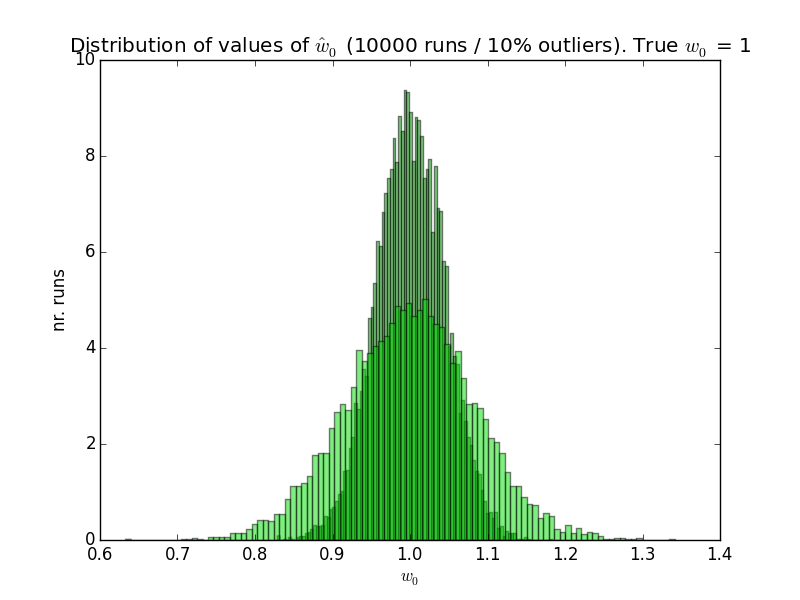
\includegraphics[width=1.0\linewidth]{chapter_lad/ols_w0_with_and_without_outliers.png}
\end{minipage}%
\begin{minipage}{.5\textwidth}
  \centering
  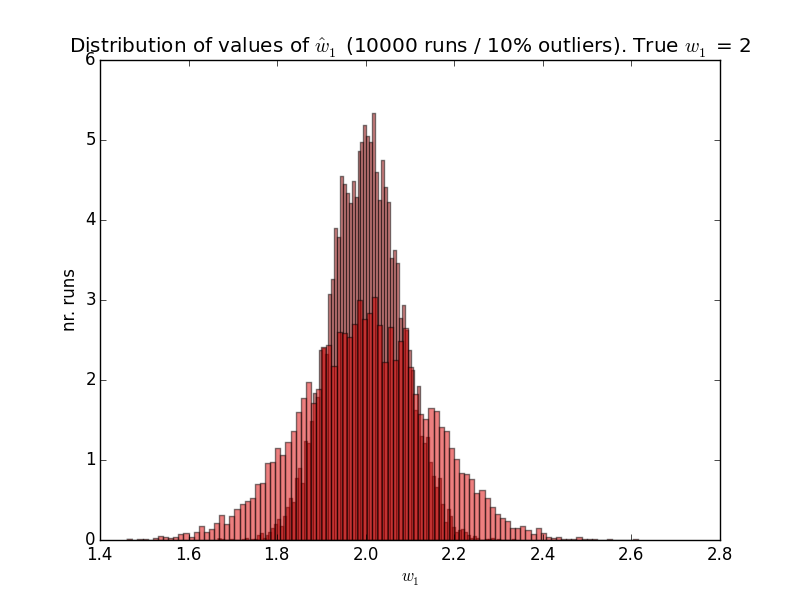
\includegraphics[width=1.0\linewidth]{chapter_lad/ols_w1_with_and_without_outliers.png}
\end{minipage}
  \label{fig.ols_estimates_with_and_with_no_outliers}
  \caption{The distribution of the estimates of the values of $w_0$ and $w_1$ for 10000 runs of OLS estimation, for two reference dataset of 500 point, one with no outliers (darker) and one with outliers (lighter)}
\end{figure}

It is very easy to see that the presence of outliers (\~ 10\% of the points) will significanlty impact the estimates $\hat{w}_0$ and $\hat{w}_1$. In the absense of outliers (Scenario 1), the values of the estimates are all concentrated around the true values, $w_0$ and $w_1$. But when outliers are present, the distribution of estimates is much more spread out around the true value, which indicates that the estimation process is not robust to such outliers.

The reason for such lack of robustness to outliers is related with the fact that the squared loss weights errors desproportionally: a few large residues may contribute much more to the overall loss value than a large number of small errors (which quadratically will tend to zero). As such, the OLS minimization process will lead to solutions that will make the resulting hyperplane pass closer to those outlier point (because they weight more on the final error) that what we would like, at the cost of sacrifying the fit for a larger set of points. Potentially, a few distant outliers may incluence the optimization so much that because of them the we sacrifice the fit for the majority of points.

There are, of course, method for removing some of these points from the trainning set prior to running the OLS procedure. But, we can also follow a totally different strategy, go back to the drawing board and formulate the problem again from the basics using a different loss function, hopefully one that does not suffer from the hypersensitivity to outliers as the squared loss does. Basically we wish to: 
\begin{equation}
\begin{aligned}
& \underset{R}{\text{minimize}} & & \mathcal{L}(Y, \hat{Y}) \\
& \text{subject to} & & \hat{Y} = X \hat{w}  
\label{eq.fundamental_minimization_problem}
\end{aligned}
\end{equation}
what if we plug a loss functions that is not the squared loss? 

\subsection{Minimizing L1 Loss}
As mentioned in Section \ref{section_loss_functions}, there are other loss functions available. The core of the Least Absolute Deviation is precisly solving the previous optimization problems when you plug in the \emph{Absolute Loss}, also known as L1 loss: 
\begin{equation}
\mathcal{L}_{L1}(Y, \hat{Y}) = \sum_n | y_i - \hat{y}_i | = \sum_n | y_i - x_i  \hat{w} |
\end{equation}
Overall the problem now becomes:
\begin{equation}
\begin{aligned}
& \underset{R}{\text{minimize}} & &  \sum_n | y_i - \hat{y}_i | = | Y - \hat{Y} |  \\
& \text{subject to} & & \hat{Y} = X \hat{w}  
\label{eq.fundamental_minimization_problem}
\end{aligned}
\end{equation}
Solving this optimization problem, however, is not as trivial as solving the OLS, and there is no closed form solution. The biggest difficulty is that there is not derivative of the absolute loss function, so there is on way of solving the equation:
\begin{equation}
\frac{\partial \mathcal{L}_{L1}(Y, \hat{Y})}{\partial \hat{w}} = 0
\end{equation}
analytically to get a closed form solution for $\hat{w}$.

So, how do we solve this minimization problem? One of possible ways is to formulate this problem as Linear Programming (LP) problem for which we can use one of many LP techniques, such as the Simplex Method. Let's start by defining $ad_i$, the \emph{deviation} for data point ($X_i$, $y_i$) as:
\begin{equation}
dv_i = |y_i - x_i \cdot \hat{w}| = |y_i - 1 \cdot w_0 - x_{i1} \cdot w_1 ... - x_{id} \cdot w_d |
\end{equation}
assuming the that the X vector has d components (including component 0 that corresponds to intersect and has value 1)
So, what we want to minimize is the sum of all these deviations
\begin{equation}
\begin{aligned}
& \underset{\hat{w}}{\text{minimize}} & &  \sum_n | dv_i | 
\label{eq.fundamental_minimization_problem_lad}
\end{aligned}
\end{equation}
which can be reformulated as:
\begin{equation}
\begin{aligned}
& \underset{\hat{w}}{\text{minimize}} &  \sum_n dv^{max}_i  & \\
& \text{subject to}                              & & dv^{max}_i > dv_i \\
&                                                        & & dv^{max}_i > - dv_i \\
\label{eq.fundamental_lad_minimization_problem_simplex}
\end{aligned}
\end{equation}

\begin{equation}
\begin{aligned}
& \underset{\hat{w}}{\text{minimize}} &  \sum_n dv^{max}_i  & \\
& \text{subject to}                              & & dv^{max}_i > y_i - 1 \cdot w_0 - x_{i1} \cdot w_1 ... - x_{di} \cdot w_d \\
&                                                        & & dv^{max}_i > - (y_i - 1 \cdot w_0 - x_{i1} \cdot w_1 ... - x_{di} \cdot w_d) \\
\label{eq.fundamental_lad_minimization_problem_simplex_expanded}
\end{aligned}
\end{equation}
It is important to understand that the last tow restrictions are equivalent to imposing that $dv^{max}_i = | dv_i |$. Suppose that $dv_i > 0$, then the first restriction dominates the second (which is necessarily satisfied if the first one is satisfied) and so we want to minimize a positive deviation, which is equivalent to minimizing $|dv_i|$. 

Suppose now that we have $dv_i < 0$. Then the second restriction, which implies minimizing the symmetric of such value (hence a positive value) dominates the first restriction (which would be necessarilty satisfied because it is negative). So, in this case, because we are changing the signs of the value, we are again minimizing a positive value. So, in both cases the value we are trying to minimize is a positive value which is the majorant of $|dv_i|$.

The advantage of the formulation presented in Equation \ref{eq.fundamental_lad_minimization_problem_simplex_expanded} is that it does not contain any absolute value operator making it equivalent to the canonical form of a linear programming problem:

\begin{equation}
\begin{aligned}
& \underset{\hat{w}}{\text{minimize}} &  B^TV = \sum b_i v_i & \\
& \text{subject to}                              & &  A^T V \ge C \Leftrightarrow \forall_j \sum a_{ji} v_i \ge c_i\\
&                                                        & & v_i \ge 0 \\
\label{eq.canonical_linear_programming}
\end{aligned}
\end{equation}

As such, we can now use any linear programming solver available to compute $\hat{w}$. One solver availalbe for Python is the CVXOPT package (see \url{http://cvxopt.org}). For the sake of completeness we present next the code required to implement Least Absolute Deviations method. 

\begin{lstlisting}
import numpy as np
from cvxopt.modeling import variable, op, sum, matrix

def solve_lad(X,Y):
  Y_cvx = matrix(Y)
  X_cvx = matrix(X)
  w_hat = variable(X.shape[1])
  ## This is where we say we wish to minimize the absolute loss
  op(sum(abs(Y_cvx - X_cvx*w_hat))).solve()
  return w_hat.value
\end{lstlisting}

The core of the code is the call to the op function, in which we basically pass the function we want to minimize and ask the solver to do all the hard work for us.


\subsection{Testing Robustness to Outliers: Take 2}
So now that we have the tools, let's revisit the previous example where we injected outliers in the trainning data and compare distribution of estimate $\hat{w}$ by using the LAD framework (i.e. under the $\mathcal{L}_{L1}$ loss).

We are going to repeat the previous experiment just changing the method used to estimate $\hat{w}$. Again, two scenarios will be considered: in Scenario 1 we have a moderate amount of noise in the data and in Scenario 2 we are injecting about 10\% of outliers (points to which we've added a much larger amount of noise). 

Figure \ref{fig.lad_estimates_with_and_with_no_outliers} shows the distributions of the estimates of $w_0$ and $w_1$ obtainined by running the Least Absolute Deviation method on 10000 experiments. We maintained the same color code (the distributions obtained for Scenario 1 are represented by darker colors).

\begin{figure}[h]
\centering
\begin{minipage}{.5\textwidth}
  \centering
  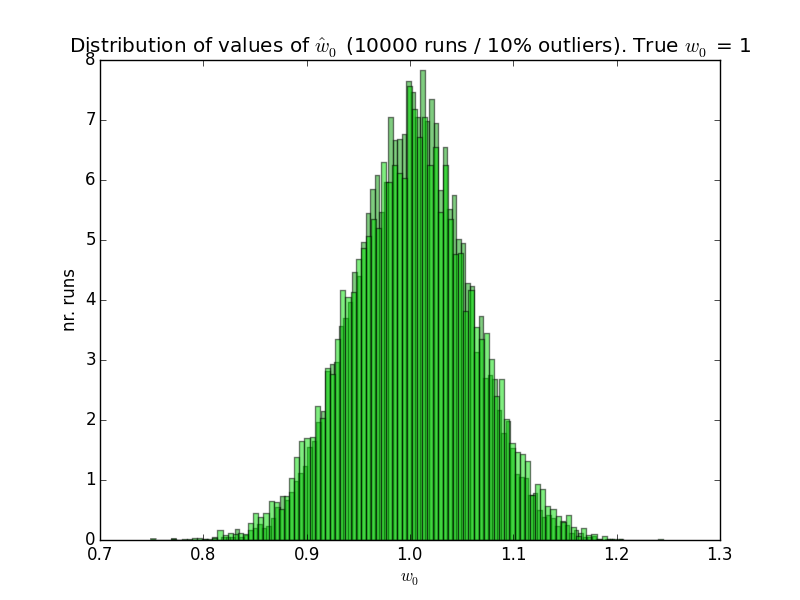
\includegraphics[width=1.0\linewidth]{chapter_lad/lad_w0_with_and_without_outliers.png}
\end{minipage}%
\begin{minipage}{.5\textwidth}
  \centering
  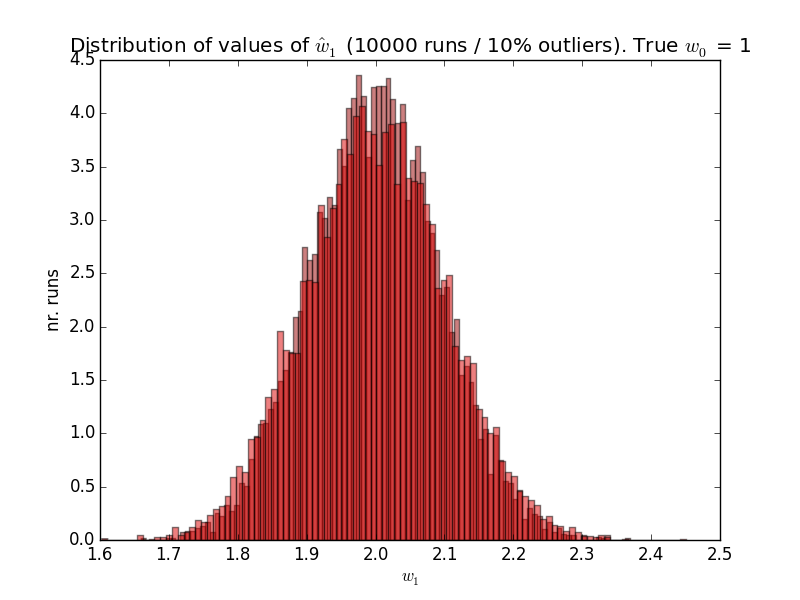
\includegraphics[width=1.0\linewidth]{chapter_lad/lad_w1_with_and_without_outliers.png}
\end{minipage}
  \label{fig.lad_estimates_with_and_with_no_outliers}
  \caption{The distribution of the estimates of the values of $w_0$ and $w_1$ for 10000 runs of LAD estimation, for two reference dataset of 500 point, one with no outliers (darker) and one with outliers (lighter)}
\end{figure}

A couple of key observations. The first one is that, just like in the OLS method, the distributions of the estimates are centred around the correct values ($w_0$ = 1 and $w_1 = 2$). So, the LAD method produces unbiased estimates and is thus a valid estimation procedure. 

The second key observation is that the OLS seems to be able to generate estimates which are much more robust to the presence of outliers. In fact, in this experiment, it is almost impossible to differentiate the distributions of the estimates with and without the presence of outliers. This is in clear contrast with the results obtained when using the OLS method, where the addition of the outliers significantly increased the variance of the distribution.

\subsection{So, what's the catch?}
When something seems too good to be true it is because it probably is. And this case, that intuition still holds because there is one big caveat that we have not addressed: computational complexity. But let's first go back to the OLS method:

\begin{lstlisting}
import numpy as np

## Given our observed X and Y, let's solve the OLS to
## estimate w_hat, which is given by:
##
## w_hat = (X^T X)^-{1} X^T Y
##

def solve_ols(X,Y):
  XtX = X.transpose().dot(X)
  XtY = X.transpose().dot(Y)
  w_hat = np.linalg.inv(XtX).dot(XtY)
  return w_hat
\end{lstlisting}


We can see that we are dealing with pretty simple matrix operations. Matrix multiplication runs in O($N^2$), and matrix inversion runs a little bit faster than O($N^3$). The matrix inversion can potentially be the bottleneck, but in fact it may not even be since the inversion is made on $X^TX$ which is a d x d matrix, with d being the dimentinality of the X vectors, i.e. the number of features used (plus 1 for the intercept). This gives us a cost of $O(d^3)$ but, unless d is very high, this inversion does not actually represent the bottleneck of the computation. 

Very frequently, the actual cost be dominated by the dimension related with the number of (X,Y) data point, n. Usually $n \gg d$, but the number of examples will ''only" impact the matrix multiplication, which means that if the number of features is small, the complexity of the OLS method will be dominated by O($n^2$). This baiscally means that is not too bad to run OLS even for relatively large dataset. 

So, what about the linear programming solver? The solver runs a variation of the Simplex algorithm, whose computational complexity \emph{tends} to be on the order O($N^3$) on the number of points. This is already much worse than OLS if the number of X Y points in our problem is large. In fact, the situaiton is even worse because there are not guarantees that the solver will actually reach a solution in less than an exponential number of steps. Compared to this, the OLS methods is blazing fast (it's just O($n^2$)!!).

\subsection{Thinking about Implicit Assumptions that come with Loss Functions}
So, the L1 loss seems lead to estimation processes that are more robust to noise than the L2 loss. The question is way? The quick answer for this question is that the L2 loss overpenalizes "distant points" and because of that such distant points tend to exert a lot of influence on the solution of the optimization problem and thus make the resulting linear model pass as close as possible to them. As a consequence, in the presence of outliers, the model will fit too much to outlier points even at the cost of misfitting the good data points. 

On the other hand the L1 loss treats distant points just as linearly more distant than closer points. Therefore, it is very hard for a few distant outliers to outweigh the vast majority of good points, and the resulting model with therefore fit the majority of points and practically ``ignore" the outliers.

That is a perfectly valid answer but let's revert the question: by chosing one or the other loss function, what are we implictly saying about the properties of the noise that we believe to be affecting the data. In other words, when we chose the L2 loss or L1 loss, what are we implicitly stating about what we believe to be the probability distribution of the noise?


